\chapter{NOTICIAS PODCAST}

\section{Que son los feed de noticias}

RSS y Atom son XML formatos para mensajes y otra informacio\'{o}n que es actualizada frecuentemente.
los documentos que son escritos en estos formatos son llamados "newfeeds" or "feed".\cite{einstein}



\section{RSS Requerimientos}

Se tiene como significado de RSS como ser: "RDF Site Summary", "Rich Site Summary", o "Really Simple Syndication",
"Atom", mas que todo sincronizaci\'{o}n de web tecnologias.\cite{dirac}

\scriptsize

\begin{flushleft}

La abreviatura RSS se ha consolidado como el t\'{e}rmino colectivo para estos newfeed formatos. El nombre "RSS"
abarca una serie de tecnolog\'{i}as estrechamente conectadas que identifican y encontrar actualizada o informaci\'{o}n
actualizada en la Web, y mostrar e intercambio esa informaci\'{o}n. El termino RSS desarrollado a partir de una abreviatura que ese puede interpretar de diferentes formas: las tres cartas, dependiendo de su interpretaci\'{o}n,
representan "RDF Site Resumen", "Rich Site Summary", o "Really Simple Syndication", "Atom" es el nombre de un intento
de formular RSS de una forma nueva, m\'{a}s precisamente y en estrecha sincronizaci\'{o}n con otras tecnolog\'{i}as web-actualizados.

\end{flushleft}

\normalsize

\section{Semantica: El Modelo RSS}

El functiones b\'{a}sicas comunes de los formatos de sindicaci\'{o}n se pueden dividir en cuatro categor\'{i}as.

\begin{itemize}

\item \textbf{Arquitectura:} estructura de informaci\'{o}n.

\item \textbf{Contenido:} descripci\'{o}n y reproducci\'{o}n de informaci\'{o}n.

\item \textbf{Identificaci\'{o}n y vinculaci\'{o}n:} trasladarse a otra informaci\'{o}n sobre la Web.

\item \textbf{Metadatos:} descripci\'{o}n de importantes caracteristicas de la informaci\'{o}n.

\end{itemize}

Si las diferentes versiones RSS, ciertamente la semantica es lo mas importante de los lenguages en similar.

\scriptsize

\begin{flushleft}

Incluso si las diferentes versiones RSS difieren claramente uno de otros, la sem\'{a}ntica de la mayor\'{i}a
de las caracter'{i}sticas importantes de la lengua son similares. El modelo de una colecci\'{o}n de actualizado
objetos de informaci\'{o}n que pertenecen a un recurso que es identificable en la Web forma la base de datos los
vocabularios de sindicaci\'{o}n. La alimentaci\'{o}n de documentos es una instant\'{a}nea del recurso.

\end{flushleft}

\normalsize

\section{Sintaxis: RSS como XML formato}

Para muchos desarrolladores "XML" y "RSS"son sinominos. Se utiliza ambas tecnologias para el intercambios de informaci\'{o}n
en la Web.

\scriptsize

Muchos sitios web de identificar sus fuentes de noticias a trav\'{e}s de un bot\'{o}n de color naranja marcado "XML". Para muchos
usuarios, y tambien para muchos desarrolladores "XML" y "RSS" son sin\'{o}nimos. De hecho, todas las versiones del formato RSS y
Atom son XML aplicaciones. Desde XML en s\'{i} es un metalenguage para definir idiomas par el intercambio de informaci\'{o} en la
Web, los formatos de fuentes son tambi\'{e}n a menudo se llama "dialectos XML" o "XML vocabularios". A la fecha, RSS es el vocabulario, 
excepto XML de mayor \'{e}xito para tal XHTML, la versi\'{o}n XML de HTML.

\normalsize

\section{Las versiones de RSS y Atom: su evoluci\'{o}n y el futuro}
Si se utiliza una version de RSS esta se tiene que especificar con la version con la que se tiene
que trabajar o simplemente utilizar Atom.

\scriptsize

Si se utilizo el t\'{e}rmino "RSS" en este libro sin el n\'{u}mero de versi'{o}n, act'{u}a como un colectivo
t\'{e}rmino para "las diferentes versiones de RSS y Atom" como un grupo, es decir, como sin'{o}nimo de "Formato
de alimentaci\'{o}n". si yo hablo de uno de estos formatos, yo uso "RSS" con una versi'{o}n n\'{u}mero o el nombre
"Atom".

\normalsize 

\section{RSS 0.90}

Con RSS es posible integrar titulos desde otros sitios en la portada. Los usuarios deberian personalizar
y suscribirse a un numero de canales que ofrece RSS.

\scriptsize

RSS fue inicialmente una abreviatura de "RDS Site Summary" (Para obtener informaci\'{o}n acerca de RSS como)
"RDF Site Summary" consulte el Cap\'{i}tulo 3, Para una explicaci\'{o}n detallada del t\'{e}rmino, ver secci\'{o}n
3.1 RDF Fundamentos) Con RSS, es posible integrar los titulares de otros sitios con enlaces a estos sitios en el 
portal. El usuario puede personalizar el portal y suscribirse a un n\'{u}mero de sitios que ofrecen datos RSS.
De esta manera, My Netscape ten\'{i}a a su disposici\'{o}n una gran cantidad de contenidos adicional, que mantiene
a los usuarios en el sitio ya; los proveedores de datos RSS recibida tr\'{a}fico en el objetivo adicional m\'{a}s
importante de muchos sitios web en los tiempos de la boom de las punto-com. Puesta que es f\'{a}cil de convertir 
RSS a HTML. otros sitios pronto empezaron a utilizar la misma tecnolog\'{i}a. Slashdot pronto utiliza RSS en lugar
de su propio formato de t\'{i}tulo, y herramientas fueron desarrolladas para crear y el proceso de RSS en los 
lenguages de programaci\'{o}n comunes.

\normalsize

\subsection{RSS 0.91}

Cuando Netscape libera la especificacion RSS 0.91, todas las referencias de RDf fueron removidas.
Desde RDF no fue parte de la especificación, los acronimos RSS no se tenia sentido ya. Dave Winer
declaro "No hay consenso sobre lo que RSS significa, así  que no es un acrónimo, es un nombre".
En julio 2000, el libero su propia versi\'{o}n de RSS 0.91. El reformatero el documento para hacer
este mas f\'{a}cil.

\subsection{Los elementos de RSS 0.91}

La definitiva fuente de informaci\'{o}n respecto RSS 0.91 es la especificación de esta misma, pero 
para su conveniencias nosotros tenemos un diagrama resumido. Cada caja en el diagrama representa
un elemento XML, y una fila indica contención.

Nosotros tenemos el <rss>, <channel>, y <item>, pero algunos nuevos elementos aquí merecen mensión:

\begin{itemize}

\item <image> - Este logotipo permite un sitio web para especificar una imagen de icono o logotipo para
se mostrara cuando se muestra el suministro de noticias en un lector de noticias o en otra pagina web.

\item <lastBuildDate> - Este elemento especifica la última vez que cualquier elemento de la noticias los
cambios de alimentación.

\item <pubDate> - Este elemento especifica el tiempo que el feed de noticias fue el último publicado, utilizando
es RFC 822, formato de fecha. Tenga en cuenta que el canal en si tiene una fecha de publicación, pero los
elementos individuales en el feed de noticias no lo hacen. Eso es un sería limitación para las aplicaciones
que se basan sobre el tema data de ordenar los elementos.

\item <textInput> - Otro elemento rara vez usado, <textInput> ofrece una manera para que un editor permita al
lector a consultar el sitio web de la editorial.

\item <skipDays> y <skipHours> - Estos elementos permiten a los editores para especificar los momentos en los
que es poco probable un flujo que se actualice. La mayoria noticias lectores de feeds ingnoran estos
valores.

\end{itemize}

Volvamos a nuestra lección de historia, recogiendo la historia con RSS 1.0

\begin{figure}[!htb]
\centering
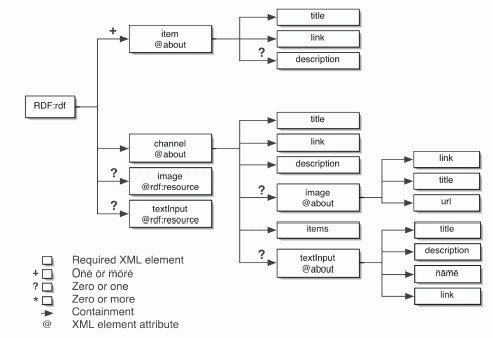
\includegraphics[scale=0.5]{rss1}
\caption{los elementos XML que componen RSS 0.91}
\end{figure}


\section{Los elementos de RSS 1.0}

Comparando los RSS 0.91 y RSS 1.0 diagramas, tu puedes ver los formatos son significativos diferentes.
Aqui son las palabras diferentes:

\begin{itemize}

\item Un típico flujo RS 1.0 es más largo y más complejo, pero no lo hace incluir tantos metadatos como el
equivalente RSS 0.91 newfeed.

\item RSS 1.0 es más complejo, pero sólo porque es más flexible y extensible.

\item El elemento raíz es <RDF:rdf> en lugar de <rss>.

\item Las noticias existen como hijos de elemento raíz del documento y no como hijos del elemento <channel>,
como lo hacen en RSS 0.91.

\item Las noticias deben ser declaradas dentro del <channel> como recursos DRF. \par

\begin{minipage}{1.0\linewidth}
	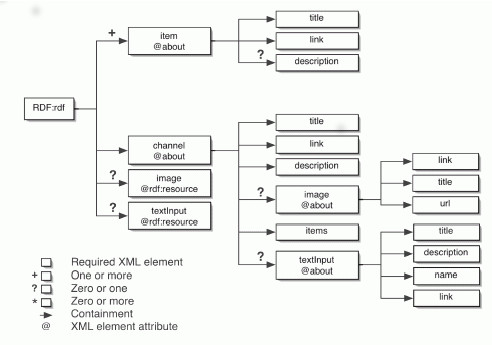
\includegraphics[scale=0.5]{rss09}
		\captionof{figure}{Los elementos XML que componen RSS 1.0}	
\end{minipage}

\item <image> y <textinput> elementos deberian ser declarado dentro los <RDF:rdf> elementos son RDF
si han de ser incluidos dentro de la <channel> elemento.

\item Muchos elementos de metadatos, tales como  <pubDate>, <lastBuild-Time>, <skipDays>,
<skipHours>, <managingEditor>, y <webMaster> faltan del para. Estos se pueden añadir según sea necesario
mediante el uso de RSS 1.0 módulos, que se describen en la siguiente sección.

\end{itemize}

\section{Los elementos de RSS 2.0}

Los RSS 2.0 especificación provee un detallada descripción de cada elemento permitido en un RSS 2.0
newfeed. Tu pueden encontrar la especificación aqui  http://blogs.law.harvard.edu/tech/rss. Resumiendo
el XML que componen RSS 2.0, usando la misma notacion como nuestra previa figura, con un toque.

\begin{figure}[h]
\centering
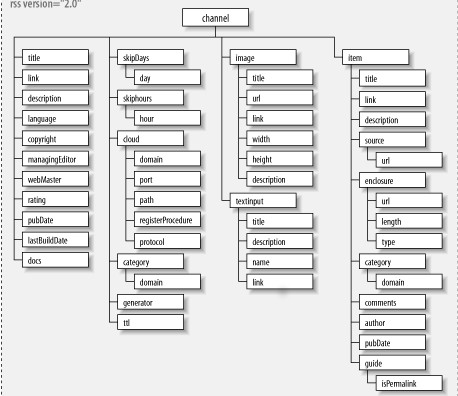
\includegraphics[scale=0.5]{rss2}
\caption{Los elementos XML que componen RSS 2.0}
\end{figure}

Algunos de los nuevos elementos aniadidos ademas de RSS 0.91 merecen explicacion:

\begin{itemize}

\item Ahora puede especificar categorías a nivel de canal o en el nivel de artículo por usando el <category>
 elemento. Se permite múltiples categorias. Si usted utiliza un sistema de taxonomía o clasificación 
 conocida, se puede observar que por especificando el URI de la taxonomía en el atributo de dominio opcional.

\item El nivel de artículo <comentarios> elemento puede ser utilizado para especificar la dirección URL de la
página de comentarios de una entrada de blog específico.

\item El nivel de artículo <guid> elemento puede utilizarse para especificar un identificador único global.
para cada elemento. A menos que especifique el atributo ispermalink="false", el GUID se considerará el 
enlace permanente a la representación web del tema newsfeed. Desafortunadamente, esto presenta la oportunidad
para la confusión por que el elemento <link> se utiliza a veces como enlace permanente al tema.

\item El nivel de artículo <author> elemento le permite especificar el correo electrónico del autor. Si deseas
especificar el nombre del autor, se puede utilizar el Dublin Core Module <dc:creator> element.

\item El nivel de artículo <enclosure> elemento puede utilizarse para adjuntar un archivo a un elemento. Para incluirlo
un archivo, debe especificar el archivo de URL, tipo de contenido, y la longitud.

\end{itemize}

\subsection{Extendiendo RSS 2.0}

Para el momento RSS 2.0 estubo liberado en Agosto 2002, todo el mundo reconocio el valor de RSS 1.0-style 
modulo de extension. Ganador decidio permitir el mismo tipo de extension a RSS. Lo hizo mediante la adición
de esta frase a la RSS 2.0 especificación: "Un RSS feed puede contener elemento que no describen en esta página,
si sólo si esos elementos se definen en un espacio de nombres"

\subsection{Las nueve versiones incompatibles de RSS}

Un influente blogger nombre Mark Pilgrim tiene que ser seguidor el desarrollador RSS de cerca, y el tiene que hacer
algunas importantes contribuciones. Trabajando con Sam Ruby, otro influente blogger, Pilgrim desarrollo servicio validacion de noticias lugar http://www.feedvalidator.org/ que maneja toda la comúnmente uso de RSS y Atom noticas
formato. 

Pilgrim señalaron que había nueve incompatibilidades versiones de RSS. Resumiendo estas incompatibles versiones y
autores, fecha y estado de cada una.

\begin{table}[h]

\centering

\begin{tabular}{>{\centering\arraybackslash}m{.1\linewidth} |>{\centering\arraybackslash}m{.2\linewidth}|>{\centering\arraybackslash}m{.1\linewidth}|>{\centering\arraybackslash}m{.2\linewidth}|>{\centering\arraybackslash}m{.4\linewidth}}
 & \textbf{Liberado por} & \textbf{Fecha} & \textbf{Estado} & \textbf{Nota} \\
\hline

\textbf{RSS 0.90} & Libby/Netscape & Enero 1999 & \textbf{Obsoleto} y rara vez se encuentra en la naturaleza & RDF- basado formato. \\
\hline

\textbf{RSS 0.91 } & Libby/Netscape & Julio 1999 & \textbf{Obsoleto} pero ampliamente usado & XML-basado con DTD; caído todos los elementos RDF; Añadido soporte para módulos. \\
\hline 

\textbf{RSS 0.91 (UserLand) } & Winer/Userland & Junio 2000 & \textbf{Obsoleto} pero ampliamente usado & caído DTD. \\
\hline 

\textbf{RSS 1.0} & RSS-DEV & Diciembre 2000 & \textbf{Viable} y ampliamente usado & RDF-basado formato nuevamente.\\
\hline

\textbf{RSS 0.92} & Winner/Userland & Diciembre 2000 & \textbf{Obsoleto} pero ampliamente usado & Contenido tipo de <description> elemento cambiado desde texto plano\\
\hline

\textbf{RSS 0.93} & Winer/Userland & Abril 2001 & \textbf{Obsoleto} y rara vez que se encuentra en la naturaleza & Aniadidp <pubDate> y <expirationDate> elementos. tambien permite multiples <enclousure> elementos por <item> \\
\hline

\textbf{RSS 0.94} & Winer/Userland & Verano 2002 & \textbf{Obsoleto} y rara vez que se encuentra en la naturaleza & eliminado <expirationDate> elemento. Especificación ya no está disponible en línea\\
\hline

\textbf{RSS 2.0} & Winer/Userland & Agosto 2002 & \textbf{Viable} y ampliamente usado. Final version de RSS & Permite adición de nuevos elementos siempre y cuando se definen por Espacio de nombres XML\\
\hline 

\textbf{RSS 2.0.1} & Winer/Harvard & Julio 2003 & Menor cambio a RSS 2.0 & Agregado elemento <rating>\\
\hline 

\end{tabular}

\caption{Las nueve versiones incompatibles de RSS}

\end{table}

Para más información en cada una de estas versiones de RSS, ver la especificaciones encontradas sobre la Web 
en las siguientes direcciones:

\begin{itemize}

\item RSS 0.90 - http://www.purplepages.ie/RSS/netscape/rss0.90.html
\item RSS 0.91 (Netscape) - http://my.netscape.com/publish/formats/rss-spec-0.91.html
\item RSS 0.91 (UserLand) - http://backend.userland.com/rss091
\item RSS 0.92 - http://backend.userland.com/rss092
\item RSS 0.93 - http://backend.userland.com/rss093
\item RSS 0.94 - No esta disponible en linea.
\item RSS 1.0 - http://web.resource.org/rss/1.0/spec
\item RSS 2.0 - No disponible en linea.
\item RSS 2.0.1 - http://blogs.law.harvard.edu/tech/rss

\end{itemize}

\section{El nuevo estandar: Atom}

En 2003, un grupo de bloggers que eran disolucionados con el estado de las noticias y publicación estandar API
se unieron para crear un nuevo estandar. cual deberia despuesser conocido como Atom. Querian empezar de nuevo y
hacer las cosas bien esta vez. Debido a que el grupo fue dirigido por los bloggers de renombre y XML expertos
Joe Gregorio, Mark Pilgrim, y Sam Ruby, atraco de la atención y participacion de los principales dessarrolladores
de servidores de blog.

Si piensas Atom es una mejora sobre RSS o solamente otro formato, como un aplicación de blog usted 
tendra que aprender Atom. Todo el mayor servidor blog si soporta Atom ahora o tiene planes para hacer, y Blogger.com,
uno de los largos servicios blogging, ofrece solo Atom noticias - no RSS.

\subsection{Construcciones comunes Atom}

Atom define un numero de comunes constructores, atributos, y elementos que son reusados a lo largo del formato.
El mas significante son fechas, textos y personas. El contructor de texto y personas requiere explicación


\textbf{\textit{Constructor Texto}}

Un constructor de texto es un elemento que contiene texto. La manera del texto almacenado es indicando
por un tipo de atributo. Si el tipo de atributo es texto "text", los elementos contienen un plan
texto y no marcado de algun tipo. Si el tipo es "xhtml", los elementos continen sin escapar XHTML marcado
en el formulario de XHTML XML elementos y texto.

\begin{minipage}[t]{0.4\textwidth}

\begin{center}

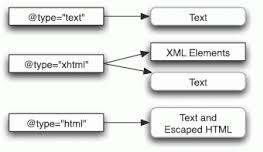
\includegraphics[scale=0.7]{textConstruct}
\captionof{figure}{Constructor de texto}

\end{center}

\end{minipage}

\textbf{\textit{Constructor Persona}}

Algunos constructores involucran mas que un XML elementos. Por ejemplo, Atom define un constructor de 
persona que es usado para representar autores y contribuyentes, como es

\begin{minipage}{0.5\textwidth}
\centering
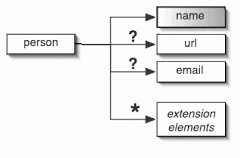
\includegraphics[scale=0.7]{personConstruct}
\captionof{figure}{Constructor de Persona}
\end{minipage}

\subsection{Los elementos de Atom}

Nosotros tenemos usado la notación <<text>>, <<person>>, y <<fecha>> a indicar cuales elementos son constructores
comunes. Requeridos elementos son compartidos.

\begin{figure}[!ht]
\centering
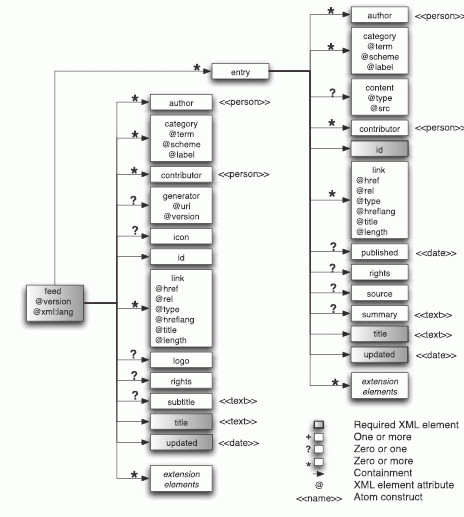
\includegraphics[scale=0.6]{elementsXML}
\caption{Los elementos XML que conforman un servicio de noticias Atom}
\end{figure}

Algunos requisitos importantes no son evidentes a partir de este diagrama formato Atom, Por lo tanto permiteme
revisar ellos. Primero, el nivel feed requisito.

\begin{itemize}

\item El feed debe contener un <id> elemento.
\item El feed debe contener un <link> con rel="self" que contiene un enlace to el feed mismo. Esto hace posible para
un programa, cual puede tener solo una copia de un documento de noticias, a encontrar la URL de las noticias.
\item El feed debe incluir un solo enlace, significando un <link> elemento con rel="alternate" - tipicamente un enlace
alternativo de un alimento hace referencia a una alternativa representación de la alimentación.
\item El autor debe ser especifico lugar el nivel feed o en cada individual entrada.

\end{itemize}

Y ahora, en cada nivel requiere.

\begin{itemize}

\item Cada entrada debe contener un <id> elemento.
\item Si la entrada no tienen un <content> elemento, deberia tener una alternativo enlace. Un enlace alternativo es su enalce
permanente, un enlace permanente entradas representacion web.
\item Un enlace puede tener multiples enlaces alternativos para diferentes lenguajes y tipos de contenidos, pero una entrada
deberia no contener mas que una enlace alternativo para cada combinacion de languages y tipo de contenido.
\item La entrada deberia incluir un <summary> elemento si el contenido es no facilmente leible, por ejemplo es no <content> 
elemento, el <content> elemento contiene algun otro texto, o el <content> referencia de elementos contenido en otros lugares.

\end{itemize}

\subsection{Podcasting con Atom}

Podcasting originado como una caracteristica de RSS, pero a medida que el mundo se mueve Atom como el nuevo estándar.
Los podcasters también lo hará - y para buenas razones. Atom puede soportar podacsting a travez del elemento <link>.
Como es el caso con RSS 2.0-basado podcasts, usted puedes tener solo un podcast por entrada. Pero con Atom, tu puedes
tener diferentes representacion por cada lenguage y por cada tipo de contenido. Por ejemplo, si usted quiere hacer un
podcast disponible en Ingles y German y en ambos mp3 y WMV formatos, usted puede hacer algo parecido a esto:

<link href=”http://example.com/podcasts/show001-usenglish.mpg”
rel=”enclosure” hreflang=”en-US” length=”21472922” type=”audio/mpg”/>

<link href=”http://example.com/podcasts/show001-usenglish.wmv”
rel=”enclosure” hreflang=”en-US” length=”23889921” type=”audio/wmv”/>

<link href=”http://example.com/podcasts/show001-german.mp3”
rel=”enclosure” hreflang=”de-DE” length=”20032879” type=”audio/mpg”/>

<link href=”http://example.com/podcasts/show001-german.wmv”
rel=”enclosure” hreflang=”de-DE” length=”19907766” type=”audio/wmv”/>

\begin{figure}[!htb]
\centering
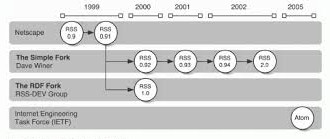
\includegraphics[scale=0.8]{newsFeed}
\caption{Newfeed árbol formato}
\end{figure}